\documentclass{article}
\usepackage{graphicx}
\usepackage[T1]{fontenc}
\usepackage{tocloft}
\usepackage{caption}
\usepackage{hyperref}
\usepackage{booktabs}
\usepackage{listings}
\usepackage{pdfpages}
\usepackage{pdflscape}
\usepackage{textpos}
\usepackage{scrhack}
\usepackage{xcolor}
\usepackage{float}
\usepackage{longtable}
\usepackage{enumitem}
\usepackage{tasks}
\usepackage{tabularx}
\usepackage{titlesec}
\usepackage{listing}
\usepackage{graphicx} 
\usepackage{geometry}
\usepackage{amsmath}

\geometry{a4paper, margin=1in}
\lstset{basicstyle=\ttfamily, breaklines=true, showstringspaces=false, commentstyle=\color{gray}}


\titleformat{\paragraph}
{\normalfont\normalsize\bfseries}{\theparagraph}{1em}{}
\titlespacing*{\paragraph}
{0pt}{3.25ex plus 1ex minus .2ex}{1.5ex plus .2ex}

\title{Internet of Things}
\author{%
Rishabh Tiwari - rishabh.tiwari@mail.polimi.it - 10987397 \and
Author Two - author.two@mail.polimi.it - 12345678 \and
Author Three - author.three@mail.polimi.it - 87654321
}
\date{February 2024}

\begin{document}
\begin{titlepage}
    \centering
    {\scshape\large AY 2023/2024 \par}
    \vfill
    
\includegraphics[width=150pt]{Images/PolimiLogo.png}\par\vspace{1cm}
    {\scshape\LARGE Politecnico di Milano \par}
    \vspace{1.5cm}
    {\huge\bfseries Internet of Things Challenge - 3\par}
    \vspace{2cm}
    {\Large \begin{tabular}{c}
    Rishabh Tiwari - rishabh.tiwari@mail.polimi.it - 10987397\\
    Marcos V. Firmino P. - marcosvinicius.firmino@mail.polimi.it
 - 10914211\\
    Alexander Stephan - alexander.stephan@mail.polimi.it - 10932707
    \end{tabular}\par}
    \vfill
    {\large Professor\par
        Redondi Alessandro \textsc{Enrico Cesare}}
    \vfill
    {\large \textbf{Version 1.1}\\ \today \par}
\end{titlepage}
\hypersetup{%
    pdfborder = {0 0 0}
}
\thispagestyle{plain}
\pagenumbering{gobble}
\mbox{}
\pagenumbering{roman}
\pagenumbering{arabic}
\section{Introduction}
In this exercise, we'll be designing a Node-RED flow to manage MQTT message exchange with a local Mosquitto broker. The flow encompasses various tasks, including message publishing, subscription, processing, logging, and interaction with external services like ThingSpeak.

The tasks are outlined as follows:

\begin{itemize}
    \item Periodically publishing MQTT messages containing randomly generated IDs and timestamps, with logging in a CSV file.
    \item Subscribing to a specific MQTT topic to receive messages, calculating a value based on the received ID, and processing a CSV file accordingly.
    \item Sending MQTT publish messages based on certain conditions, with a rate limit on publication, and formatting the payload accordingly.
    \item Plotting temperature values from publish messages in a Node-RED chart and saving relevant data to a CSV file.
    \item Handling MQTT ACK messages, logging them in a CSV file, and updating a global counter, followed by updating a ThingSpeak channel.
    \item Managing message processing to ensure a limit of 80 ID messages is not exceeded.
\end{itemize}

This exercise will demonstrate proficiency in MQTT communication, data manipulation, integration with external platforms, and flow control within Node-RED.

\section{Node-red flow}

This is a print-screen of our node-red flow

\begin{figure}[htp]
    \centering
    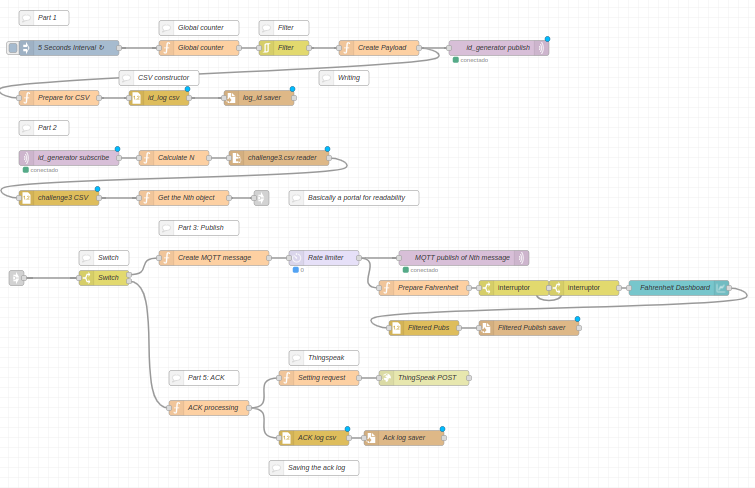
\includegraphics[width=15cm]{Images/flow.png}
    \caption{Node-red flow}
    \label{fig:galaxy}
\end{figure}

\begin{figure}[htp]
    \centering
    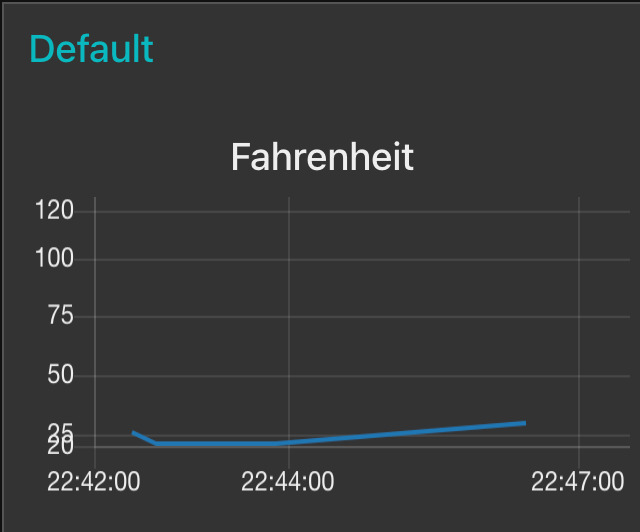
\includegraphics[width=8cm]{Images/Plot.jpg}
    \caption{Obtained Fahrenheit graph for the first couple of minutes}
    \label{fig:galaxy}
\end{figure}

\section{General Overview}
We labelled our node red flow to separate it into different sections. Here is a general overview:

\textbf{Part 1:} We inject a timestamp node to limit the messages sent to the local broker to 5 s. Then, we have some counter logic in place to make sure we don't send any messages after 80 received messages. This is done in the following function node. We save this counter in the message and the flow context. Then, we have a filter node in place. It is set to "block unless value" changes. It inspects if the counter changes, which is capped at 80. Then, we create a JSON object for message payload in the next function node, containing a random ID and a timestamp. The following MQTT out node publishes it to the topic "challenge3/id\_generator". In the "Prepare for CSV" function node, we get the counter from the flow scope to use it as No. and also create the other columns (TIMESTAMP and ID). The following CSVs node converts the created object to a CSV in Node-RED. The following "write file node" materializes the changes.

\textbf{Part 2:} In the first node, we receive the subscription from the local broker. In the next function node, we retrieve the ID from the payload and calculate it mod 7711 to get N. Then, we read the challenge3.csv file provided via Webeep.
We parse it as a csv, using a csv-node. Then, we wrote a function to retrieve the n-th element in the CSV. We subtract -1 from in the index to account for the 0 based indexing. Then, we retrieve the object using \texttt{JSON.stringify}.
Then, we use a link for readability that forwards the message to the next part.

\textbf{Part 3:} 
First, we perform string matching in the stringified JSON object for the previously retrieved row. The switch node is looking for either "ACK" or "Publish message" as the type. If we didn't receive an ACK, we create a new MQTT message. The following function node creates the actual message content. Then, we use a delay node as a rate limiter, setting the rate to 4 messages per 1 minute. Then, we publish the message using a "mqtt out node". Using this data, we create the actual plot. See the explanation of each node.

If we received an ACK node, we again process the message in a function node. Essentially, it creates a message of the right type, according to the values found in the received n-th value. Then, we create a CSV file with the "ack\_log.csv" to track the received acks. The following "write file node" materializes the CSV on our hard drive. Additionally, after receiving the ACK, we also publish it to ThingSpeak using another function node. It essentially sets the API key and the API URL. Finally, we have a "http request node" that sends the just created message via an HTTP post request.

\section{Explaining each node}

Below there is the list of all nodes and a quick description of its purpose:

\begin{itemize}
    \item 5 seconds interval: Sends the timestamp value for the next node each 5 seconds
    \item Global counter: Counts the amount of messages sent (only 80 messages allowed according to description)
    \item Filter: Filters the messages out after the 80th, thus let by only the first 80
    \item Create Payload: Create the payload of the random value generated (ID) and current timestamp
    \item id\_generator publish: MQTT node that publishes the ID and timestamp produced before
    \item Prepare for CSV: Prepares the information (ID,timestamp) to be printed into CSV
    \item id\_log CSV: Sets up the CSV file of the id\_log, for example the header
    \item log\_id saver: Actually access the file system and updates/saves the information of the log in the CSV file
    \item id\_generator subscribe: MQTT node that subscribes to the id\_generator, receiving the information (ID and timestamp)
    \item Calculate N: Given the received ID, calculates the corresponding N
    \item challenge3.csv reader: Read the file challenge3.csv
    \item challenge3 CSV: Receives the challenge3.csv data in CSV format, then convert it to JSON
    \item Get the Nth object: With the information of challenge3.csv in JSON, access the corresponding Nth message 
    \item Switch: Receives the Nth object and redirect the flow: if it contains an "ACK" or contains a "Publish Message"
    \item Create MQTT message: In case of a Pulish Message, this node reads the Nth message and extract all publish info out of it. It created the correct pair of topic-payload for each one (or more) publish messages of the Nth entry
    \item Rate limiter: Limits the rate of publication for 1 message per 4 minutes
    \item MQTT publish of Nth message: Publish each message received from the Nth object into the corresponding topic
    \item Prepare Fahrenheit: Reads the information of the message and extract the Fahrenheit value and its average, as well of preparing the message with the Fahrenheit value (if any)
    \item Interrupter: Filters out the message, and passes only if the message has a temperature in Fahrenheit
    \item Fahrenheit Dashboard: The dashboard showing the Fahrenheit information
    \item Filtered Pubs: Prepares to save the filtered message with Fahrenheit value and average
    \item Filtered Publish saver Access the file system and updates the CSV file with the temperature informatiion
    \item ACK processing: In case  of an ACK, extract the type of the ACK out of the body of the message
    \item Setting request: Sets up the HTTP request to be sent to ThingSpeak
    \item ThingSpeak POST: Perform the HTTP GET request to ThingSpeak
    \item ACK log csv: Prepares the ACK information to be saved into CSV (header for e. g.)
    \item Ack log saver: Actually access the file system and updates/saves the information of the ACKs in the CSV file
\end{itemize}

\end{document}


% 1 a) coap.code == 1 && coap.opt.uri_path contains "temperature" -> 8 (1 duplicate source port)
% 1 b) 
% coap.me.		300	IN	A	134.102.218.18
% coap.code != 2 && ip.dst == 134.102.218.18 124?
% coap && ip.dst == 134.102.218.18 && coap.opt.uri_path contains "weird" 34
% mqtt.msgtype == 3 && mqtt.qos == 2 81
% 3 clients?
% mqtt.msgtype == 8 && mqtt.msgid == 1
% broker.hivemq.com
% broker.hivemq.com.	60	IN	A	52.58.181.123
% broker.hivemq.com.	60	IN	A	18.196.194.55
% mqtt-sn && mqtt-sn.msgtype == 3 && mqtt-sn.topic == "topic6" && mqtt-sn.msgtime > "2024-03-23 13:59:00" && tcp.dstport == 1885
% 4a) mqtt.msgtype == 8 && mqtt.topic matches "[+#]"
% 

\section{Introduction}

% 1 a) coap.code == 1 && coap.opt.uri_path contains "temperature" -> 8 (1 duplicate source port)
% 1 b) 
% coap.me.		300	IN	A	134.102.218.18
% coap.code != 2 && ip.dst == 134.102.218.18 124?
% coap && ip.dst == 134.102.218.18 && coap.opt.uri_path contains "weird" 34
% mqtt.msgtype == 3 && mqtt.qos == 2 81
% 3 clients?
% mqtt.msgtype == 8 && mqtt.msgid == 1
% broker.hivemq.com
% broker.hivemq.com.	60	IN	A	52.58.181.123
% broker.hivemq.com.	60	IN	A	18.196.194.55
% mqtt-sn && mqtt-sn.msgtype == 3 && mqtt-sn.topic == "topic6" && mqtt-sn.msgtime > "2024-03-23 13:59:00" && tcp.dstport == 1885
% 4a) mqtt.msgtype == 8 && mqtt.topic matches "[+#]"
% 

\section{Traffic Analysis Exercise}
\begin{enumerate}
    \item
    \begin{enumerate}
        \item \verb|coap.code == 1 && coap.opt.uri_path contains "temperature"|
        We search for GET requests with \verb|coap.code == 1|. Then, we check whether the URI path contains the string "temperature". As specified via Webeep, clients are specified by their source port. We only observe one duplicate port, namely, 48049, therefore we count 8 clients, which made 9 requests in total.
        \item We filter for CoAP responses with the following destination ports: 
        \texttt{coap \&\& coap.code >= 65 \&\& coap.code <= 165 \&\& (udp.dstport == 55898 || udp.dstport == 33677 || udp.dstport == 51812 || udp.dstport == 48049 || udp.dstport == 52276 || udp.dstport == 48645 || udp.dstport == 52247 || udp.dstport == 41264)}. Then, we sort by length. We find the following, the message ID: 10589
    \end{enumerate}
     \item
    \begin{enumerate}
        \item First, we determine the IP of the website. This can be easily done using the \texttt{dig} utility on Linux. We get the IP 134.102.218.18.
        Then, we scan for the tokens of POST requests to this IP. We retrieve them from an exported CSV.
        Then, we can filter for response codes in the range from 100 to 200 for these tokens.
        \item 4
        % coap.code == 2 && ip.dst == 134.102.218.18 && coap.opt.uri_path contains "weird"
    \end{enumerate}
         \item
    \begin{enumerate}
        \item 30 Query = \verb|mqtt.msgtype == 3 && mqtt.qos == 2 && ip.dst == 127.0.0.1|
        \item \begin{enumerate} %Using the same string as above and filtering manually
            \item 51523
            \item 44887
            \item 32965
            \item 51524
            \item 51525
        \end{enumerate}
        \item Query = \verb|mqtt.msgtype == 8 \&\& ip.dst == 127.0.0.1|
        a
    \end{enumerate}
    \item 
       \begin{enumerate}
            \item \verb|mqtt.msgtype == 8 && (mqtt.topic contains "+" or mqtt.topic contains "#") && ip.src != 127.0.0.1| $\Rightarrow$ 4
            \item 2
            %296	60.690118129	10.0.2.15	91.121.93.94	MQTT	87	Subscribe Request (id=6) [metaverse/+/area0/light]	37419	1883
            % 551	69.497641433	10.0.2.15	3.65.168.153	MQTT	90	Subscribe Request (id=5) [metaverse/facility4/+/light]	59385	1883
    \end{enumerate}
    \item Extract a CSV of messages with length < 15 and specific mqtt version
        % mqtt.clientid_len < 15 - only connect messages
        %mqtt.msgtype == 2 && (ip.src == 127.0.0.1 || ip.src == 10.0.2.15) 
        % (ip.dst == 10.0.2.15 || ip.dst == 127.0.0.1 )&& (mqtt.msgtype == 4 || mqtt.msgtype == 5 || mqtt.msgtype == 6 || mqtt.msgtype == 7 || mqtt.msgtype == 9)
        % mqtt.clientid_len <= 15 && mqtt.ver == 4
        % => 231
    \item % mqtt.msgtype == 8 && mqtt.msgid == 1
    \item % udp.dstport==1885 && mqttsn.topic.id == 6 && mqttsn.msg.type == 0x0c && mqttsn && !icmp

    7a - 3
    
    Reason - And the second part is no because we can see that all the publish messages are accompanied by a "ICMP 82 Destination unreachable (Port unreachable)" packet.
\end{enumerate}

\end{document}
